
\begin{document}
\pagestyle{empty}

\chapter{Comparison of mismatch repair deficiency signatures in \textit{C. elegans} and human gastrointestinal cancers}

\section{Introduction}

In this chapter, I will expand on the comparison between \textit{C.elegans} 
and human cancer data. Here I will show similarities
and differences between the signatures and features of mismatch repair deficiency in different species, 
and study the composition and origins of MMR-related mutations in cancer.

%More on the comparison across species and relevance to cancer research?

The following work was published in \textit{Genome research} in 2018 (\cite{Meier2018-qz}) in co-authorship 
with Bettina Meier and colleagues, who have conceived the study, prepared the \textit{C. elegans} data 
and suggested initial filtering, mutation rate analysis and homopolymer analysis. Final estimates for indels 
per homopolymer and extraction of mutational signatures from experimental data, as well as the comparative study 
in human cancers including signature analysis, association with indels and search for interaction factors 
were done by me.

%this is a part of the publications etc%

\todo[inline]{1 paragraph on contributions! emphasize how it is different from the paper, can re-use the figure legends, do the same for other chapters}

%%%%%%%%%%%%%%%%%%%%%%%%%%%%%%%%%%%%%%%%%%%%%%%%%%%%%%%%%%%%%%%%%%%%%%%%%%%%%%

\section{Mismatch repair deficiency in cancer}

\todo[inline]{expand on the history and on the consequences}

Mismatch repair (MMR) was one of the first DNA repair pathways to be associated with 
cancer predisposition: mutations in MMR genes are associated with hereditary non-polyposis 
colorectal cancer (HNPCC), also referred to as Lynch Syndrome (\cite{Fishel1994-pp}, 
\cite{Bronner1994-nd}, \cite{Nicolaides1994-ro}, \cite{Papadopoulos1994-zk}, \cite{Miyaki1997-ae}), 
and more severe conditions leading to high rates of different neoplasms: 
biallelic mismatch repair deficiency syndrome (bMMRD) (\cite{Durno2015-lx}), Muir-Torre syndrome 
and Turcot's syndrome (\cite{Lawes2003-zd}).

Several cancer types have a high frequency of MMR deficiency, especially so in uterine, stomach and 
colorectal cancers (\cite{Cortes-Ciriano2017-rh}). Among sporadic colorectal and gastric cancers, about 15\% 
harbour MMR defects (\cite{Funkhouser2012-uq}, \cite{Cancer_Genome_Atlas_Research_Network2014-af}), and this number is higher in uterine 
cancers (up to 33\% (\cite{Hecht2006-rs})), but much lower in other cancer types (\cite{Cortes-Ciriano2017-rh}, \cite{Bonneville2017-ge}). 

Similarly to \textit{C. elegans}, MMR deficiency in humans mainly manifests via contraction and expansion
of repetitive regions called microsatellite instability or short tandem repeats, which would normally 
be repaired by MMR machinery.
While the proofreading activity of replicative polymerases can correct a fraction of mismatches, 
in absence of MMR much more replicative errors persist in the DNA and turn into mutations during the next round of replication. In healthy human cells, replication errors arise at a rate of about 1 mutation per cell division **REF**. Upon a knockout of MMR gene, the mutation rate increases up to 100-1000 fold (**RED**).

A cancer genome 
For instance, the average point mutation rate in colorectal cancer lies in the range of Cancers generally have a higher mutation rate: MMR proficient  the average point mutation 
rate in MMR-deficient colorectal cancers was observed to be 8-11 times higher (\cite{Tomasetti2015-yn}).  

Several molecular and computational methods have been developed for identification of clinically relevant
MMR deficient phenotype (\cite{Boland1998-ma}, \cite{Buhard2006-fp}, \cite{Laghi2008-yq}, \cite{Cortes-Ciriano2017-rh}, \cite{Niu2014-pt}, \cite{Bonneville2017-ge}, \cite{Huang2015-al}, \cite{Nowak2017-vo}), 
most of which quantify the number of repeats of selected microsatellites and compare it to the status of these regions in normal tissue. 
Another typical marker used in clinic is epigenetic silencing of \textit{MLH1}, which was found to be common
in cancers with sporadic MMR deficiency and is easier to reliably detect via immunohistochemistry (\cite{Herman1998-cc},
\cite{Boissiere-Michot2016-uv}). Identification of functional MMR deficiency in tumours is
important for making decisions about treatment and prognosis, as it was 
associated with better clinical outcome (\cite{Lee2002-pu}) and better response to immunotherapy 
(\cite{Dudley2016-bm}, \cite{Le2015-fb}, \cite{Kelderman2015-xv}).

%%%%%%%%%%%%%%%%%%%%%%%%%%%%%%%%%%%%%%%%%%%%%%%%%%%%%%%%%%%%%%%%%%%%%%%%%%%%%%

\section{Mutational processes shaping gastrointestinal tumours}

\subsection{De novo extraction of mutational signatures}

The previous COSMIC mutational signature catalogue (\cite{Alexandrov2015-clock}, \cite{Forbes2015-gf}) contained 5 signatures
associated with mismatch repair: 6, 15, 20, 21 and 26. It might indicate that mismatch repair deficiency
contributes to mutagenesis via multiple mechanisms at the same time, but these signatures seemed to be
uncorrelated across cancer types (\cite{Alexandrov2015-clock}). In order to gain insights into aetiology of these
signatures, we
picked stomach and colorectal adenocarcinomas as cancer types which share tissue similarity yet carry
different mutational signatures associated with MMR deficiency.

The datasets acquired from ICGC (\url{http://icgc.org}) contained single nucleotide (SNV) and 
small indel variant calls from 215 and 289 donors, respectively. 
According to the TCGA Clinical Explorer (\cite{Lee2015-hf}), 40/215 and 63/289 samples were 
labeled as microsatellite instable-high (MSI-H), which we considered as indicator of MMR deficiency. 
The samples labelled as microsatellite instable-low (MSI-L) or 
microsatellite stable (MSS) were considered MMR proficient. 
Comparison of averaged profiles of MMR deficient samples between
the cancer types showed high similarity between the two cancer types, against the presence
of different signatures in these cancers as determined by COSMIC analysis. The cosine similarity
between them reached 0.98, with the main source of variability being the contribution of 
CpG$>$TpG (Figure \ref{STAD_COAD_MSI}). 

\begin{figure}
  \centering
  \centerline{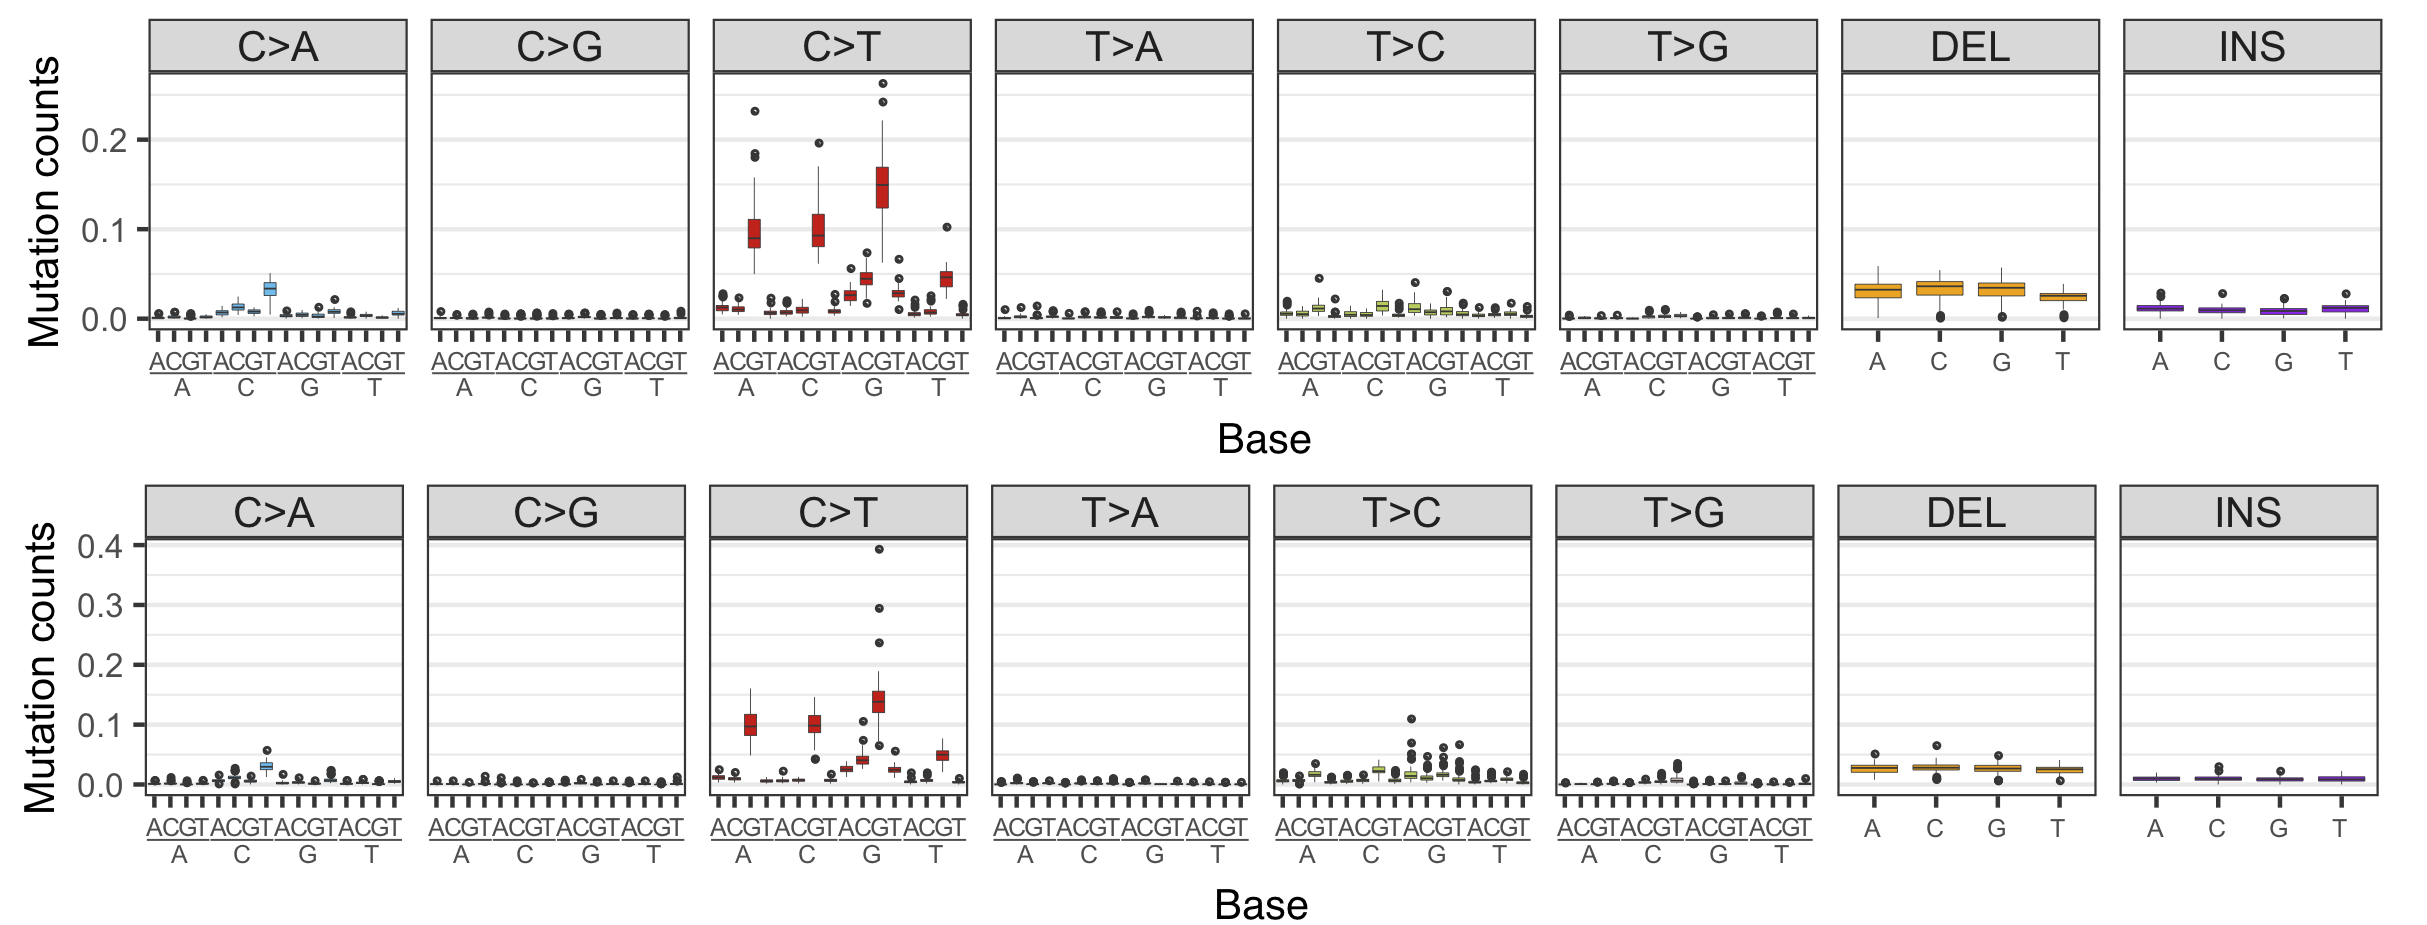
\includegraphics[width=1\textwidth]{figures/STAD_COAD_MSI_samples.png}}
  \caption{Aggregated mutational profiles of MSI samples in COAD (top) and STAD (bottom) cohorts.}
  \label{STAD_COAD_MSI}
\end{figure}

In order to analyse the signatures of mismatch repair deficiency active in these cancer types, 
we performed an unsupervised signature extraction via non-negative matrix factorisation similar 
to that initially proposed by Alexandrov in \cite{Alexandrov2013-md}. However, the initial procedure was 
performed using Frobenius norm as the loss functions minimized during the optimisation, which 
we considered not suitable for mutation count data. Hence we applied Brunet NMF with KL 
divergence \cite{Brunet2004-fm} which is equivalent to an additive Poisson model.

\begin{figure}[h]
  \centering
  \centerline{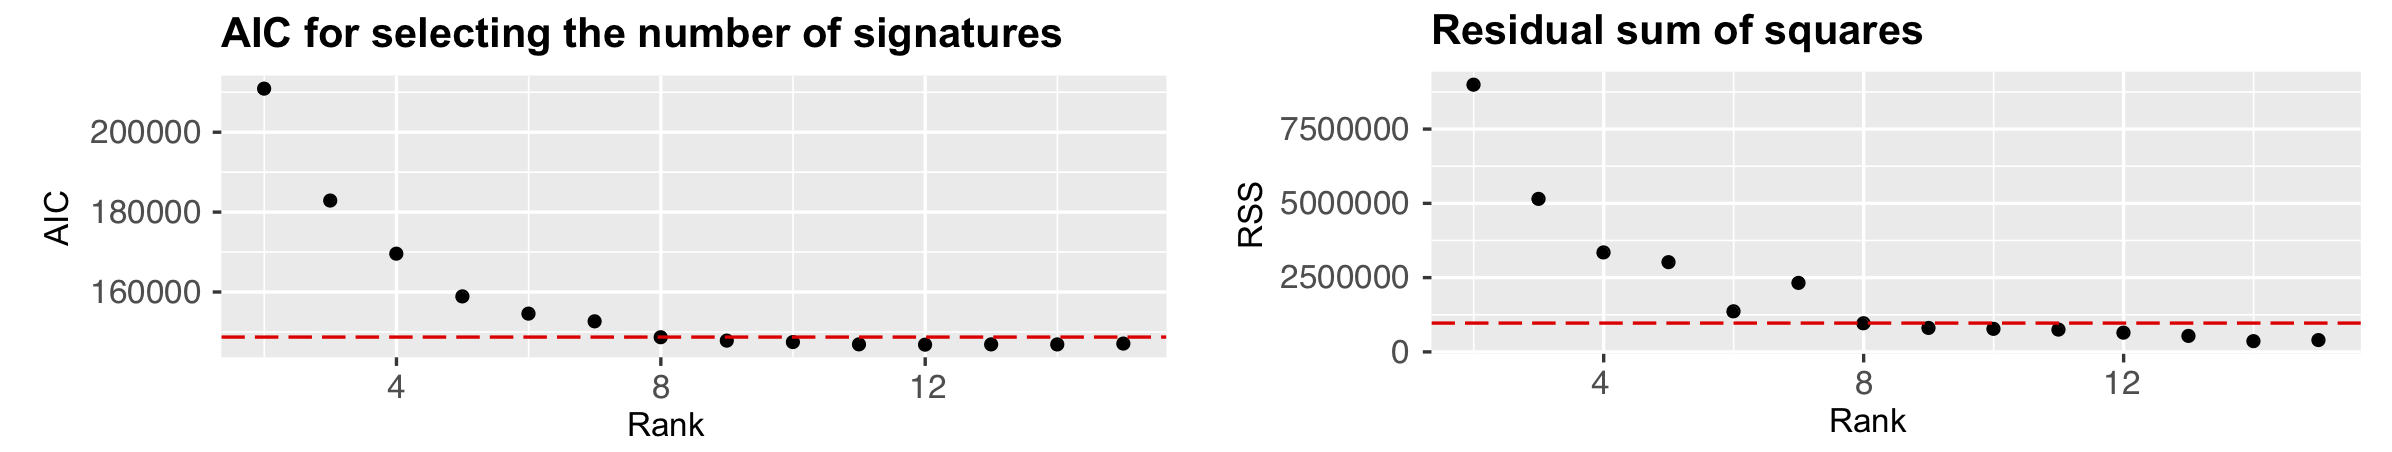
\includegraphics[width=1\textwidth]{figures/AIC_and_RSS.png}}
  \caption{AIC and RSS for detecting the number of signatures in COAD/STAD dataset.}
  \label{AIC_and_RSS}
\end{figure}


The number of signatures was chosen based on the saturation of both the Akaike 
Information Criterion (AIC) (\cite{Akaike1992-br}) and the residual sum of squares (RSS). 
The AIC is calculated as 
\[AIC = 2k \cdot (n + N) - 2\log L,\] 
where $k$ is the number of parameters (with $n$ being the number of signatures and $N$ 
being the number of samples), and $L$ is the maximized model likelihood. As the $L$ would 
naturally increase with the addition of parameters, we performed signature extraction for 
different ranks and chose the one where AIC and also RSS decrease slows down to avoid 
oversegmentation (Figure \ref{AIC_and_RSS}).

%%%%%%%%%%%%%%%%%%%%%%%%%%%%%%%%%%%%%%%%%%%%%%%%%%%%%%%%%%%%%%%%%%%%%%%%%%%%%%

\subsection{Aetiology of extracted signatures}

\todo[inline]{add similarity table}
Based on this metric, we extracted 8 mutational signatures from the combined STAD and COAD dataset
(Figure \ref{COADsigs}). Many of these signatures matched to one or more COSMIC signatures 
(Table \ref{SIMtable}), validating these results.

\begin{figure}[h]
  \centering
    \centerline{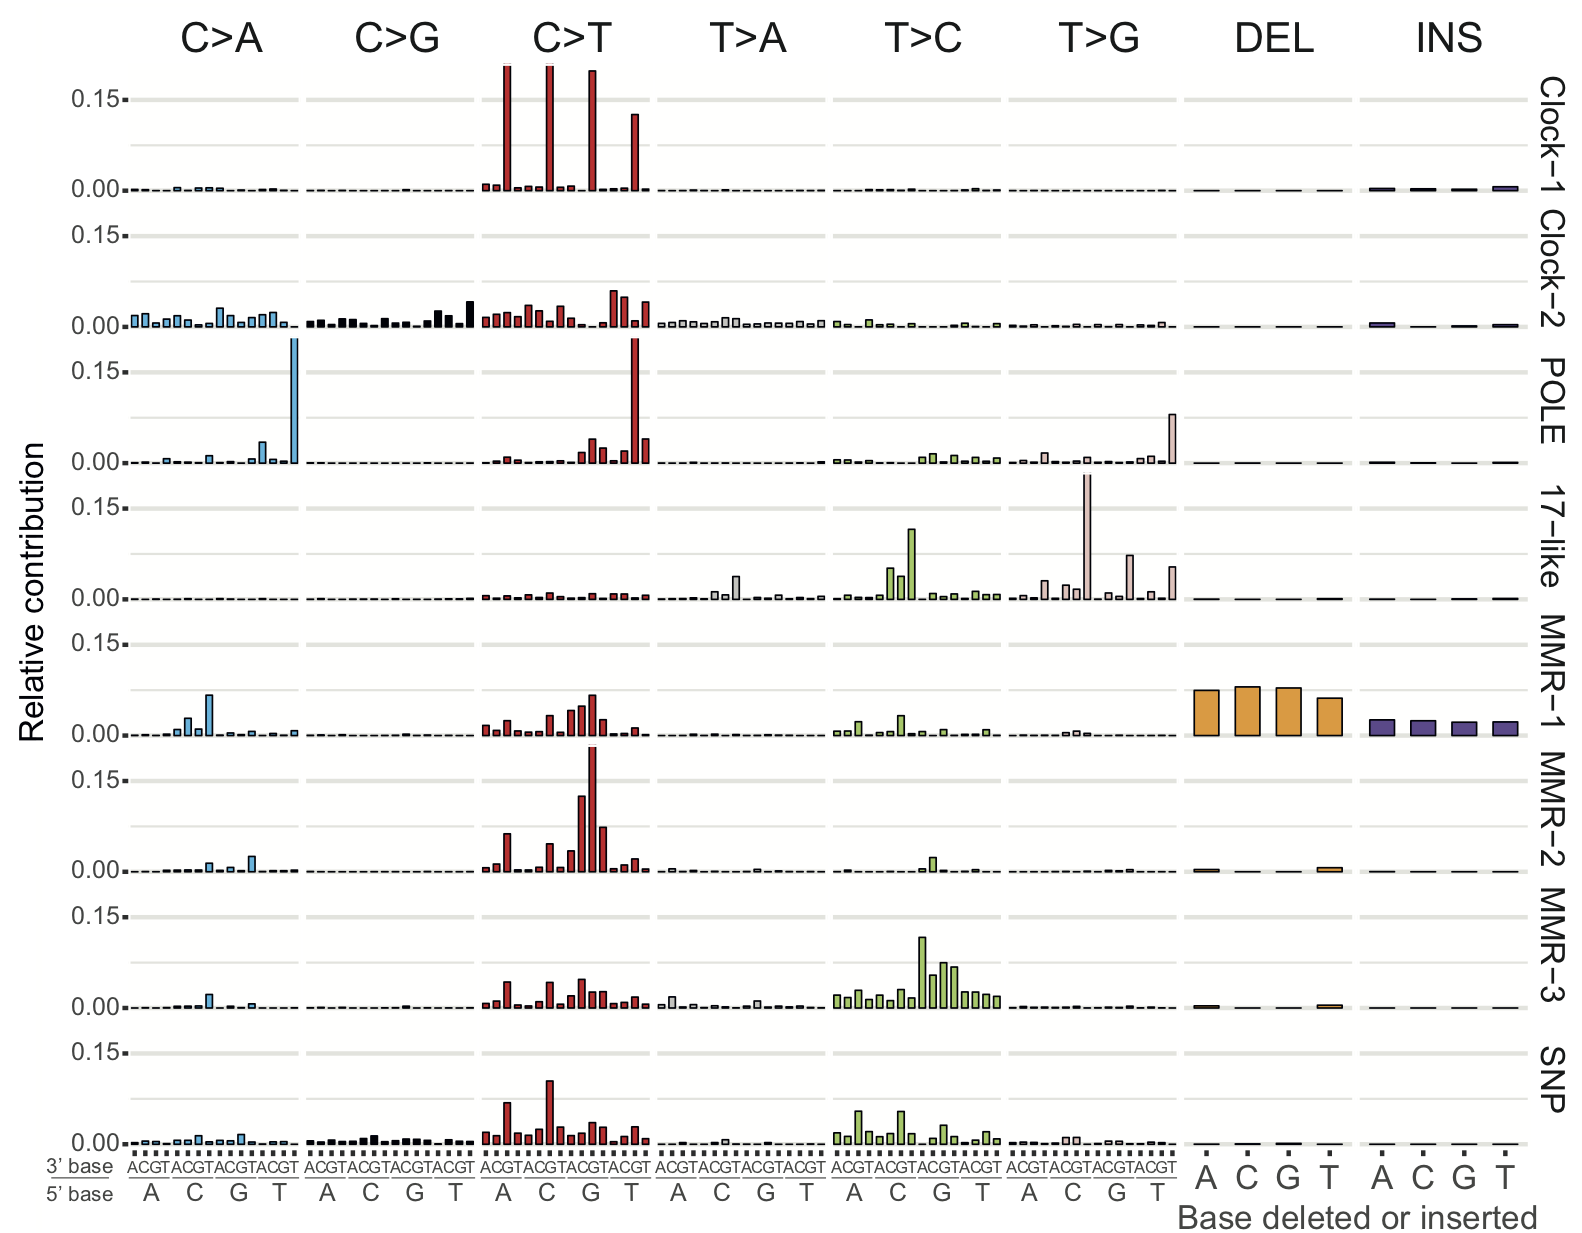
\includegraphics[width=1\textwidth]{figures/COADsigs.png}}
  \caption{Mutational signatures extracted from combined COAD/STAD dataset.}
  \label{COADsigs}
\end{figure}

For three signatures out of eight, the fraction of mutations assigned to these signatures was 
significantly higher in MMR-deficient cancers compared to proficient ones: for MMR-1 (one-tailed 
t-test p-value $= 4.7 \cdot 10^{-55}$), MMR-2 (p-value $= 1.1 \cdot 10^{-11}$) and MMR-3 
(p-value $= 6.0 \cdot 10^{-12}$). Of these, MMR-1 mostly resembled signature 20, MMR-2 - 
signature 15, and MMR-3 - signatures 21 and 26. MMR-1 signature also showed high accuracy 
in classification of MMR deficiency (AUC of 0.985).

Given the high prevalence of indels observed in \textit{C. elegans} data, we also included single
base insertions and deletions to the count matrix used for signature extraction. Interestingly, 
only one signature, MMR-1, carried all the indel information, which indicates that the profile 
of base substitutions defined by this signatures is likely to be the typical distribution of
mutations stemming from replicative errors.

\begin{wrapfigure}{r}{0.5\textwidth}
  \centering
\centerline{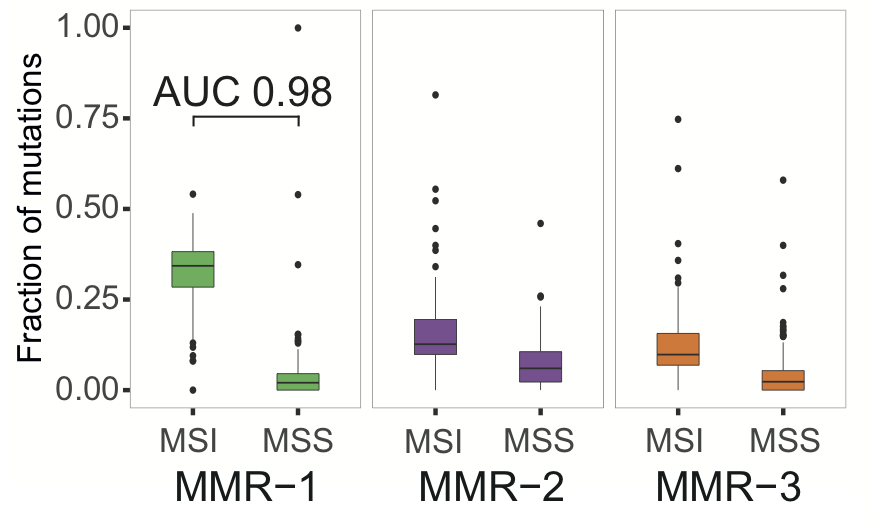
\includegraphics[width=0.5\textwidth]{figures/MSIcorr.png}}
  \caption{Association between microsatellite instability and de novo signatures MMR-1-3.}
  \label{MSIcorr}
\end{wrapfigure}

Additional signatures identified in the tumor samples were characteristic of defects in the
proofreading domain of replicative polymerase $\epsilon$ ("POLE") (\cite{Alexandrov2013-md}, \cite{Shinbrot2014-js}). 
A signature characterized by C$>$T mutations in a CpG base context, which was most likely 
to result from 5meC deamination (\cite{Alexandrov2015-clock}), was referred to as "Clock-1 (5meC)". 
"Clock 2" signatures was present in the majority of samples and likely reflected the 
background mutation rates (similar to COSMIC signature 5). "17-like" is a signature 
of unknown etiology predominantly found in stomach cancers and highly similar to 
COSMIC signature 17 (\cite{Alexandrov2013-md}).

Finally, we also identified a signature predominantly consisting of T$>$A mutation at CpG sites.
This type of mutations was present in high fraction in a limited number of samples 
(all of which were coming from the same sequencing centre), which indicated artifactual
nature of this signature. Indeed, comparing the base substitutions from the samples
carrying over 50\% of mutations assigned this signature to the set of SNPs prevalent 
in the human population (based on the dbSNP database \cite{sherry2001dbsnp}) showed a high overlap: 
mutational burden of these samples for on average 76\% (IQR 76-85\%) consisted of SNPs, 
whereas for the rest of samples this number was much lower (18\%, with IQR 0-40\%). 
In addition to that, we compared the ratio of coding and non-coding SNPs (\cite{Consortium2015-kq} ) 
and identified much lower ratio of non-synonymous to synonymous changes (0.8 with IQR 
of 0.68-0.88) across these samples than expected for cancer variants (higher than 1, 
REF), suggesting germline nature of these variants. Hence, this signature 
was referred to as "SNP" and considered as an artifact.

\begin{figure}
  \centering
\centerline{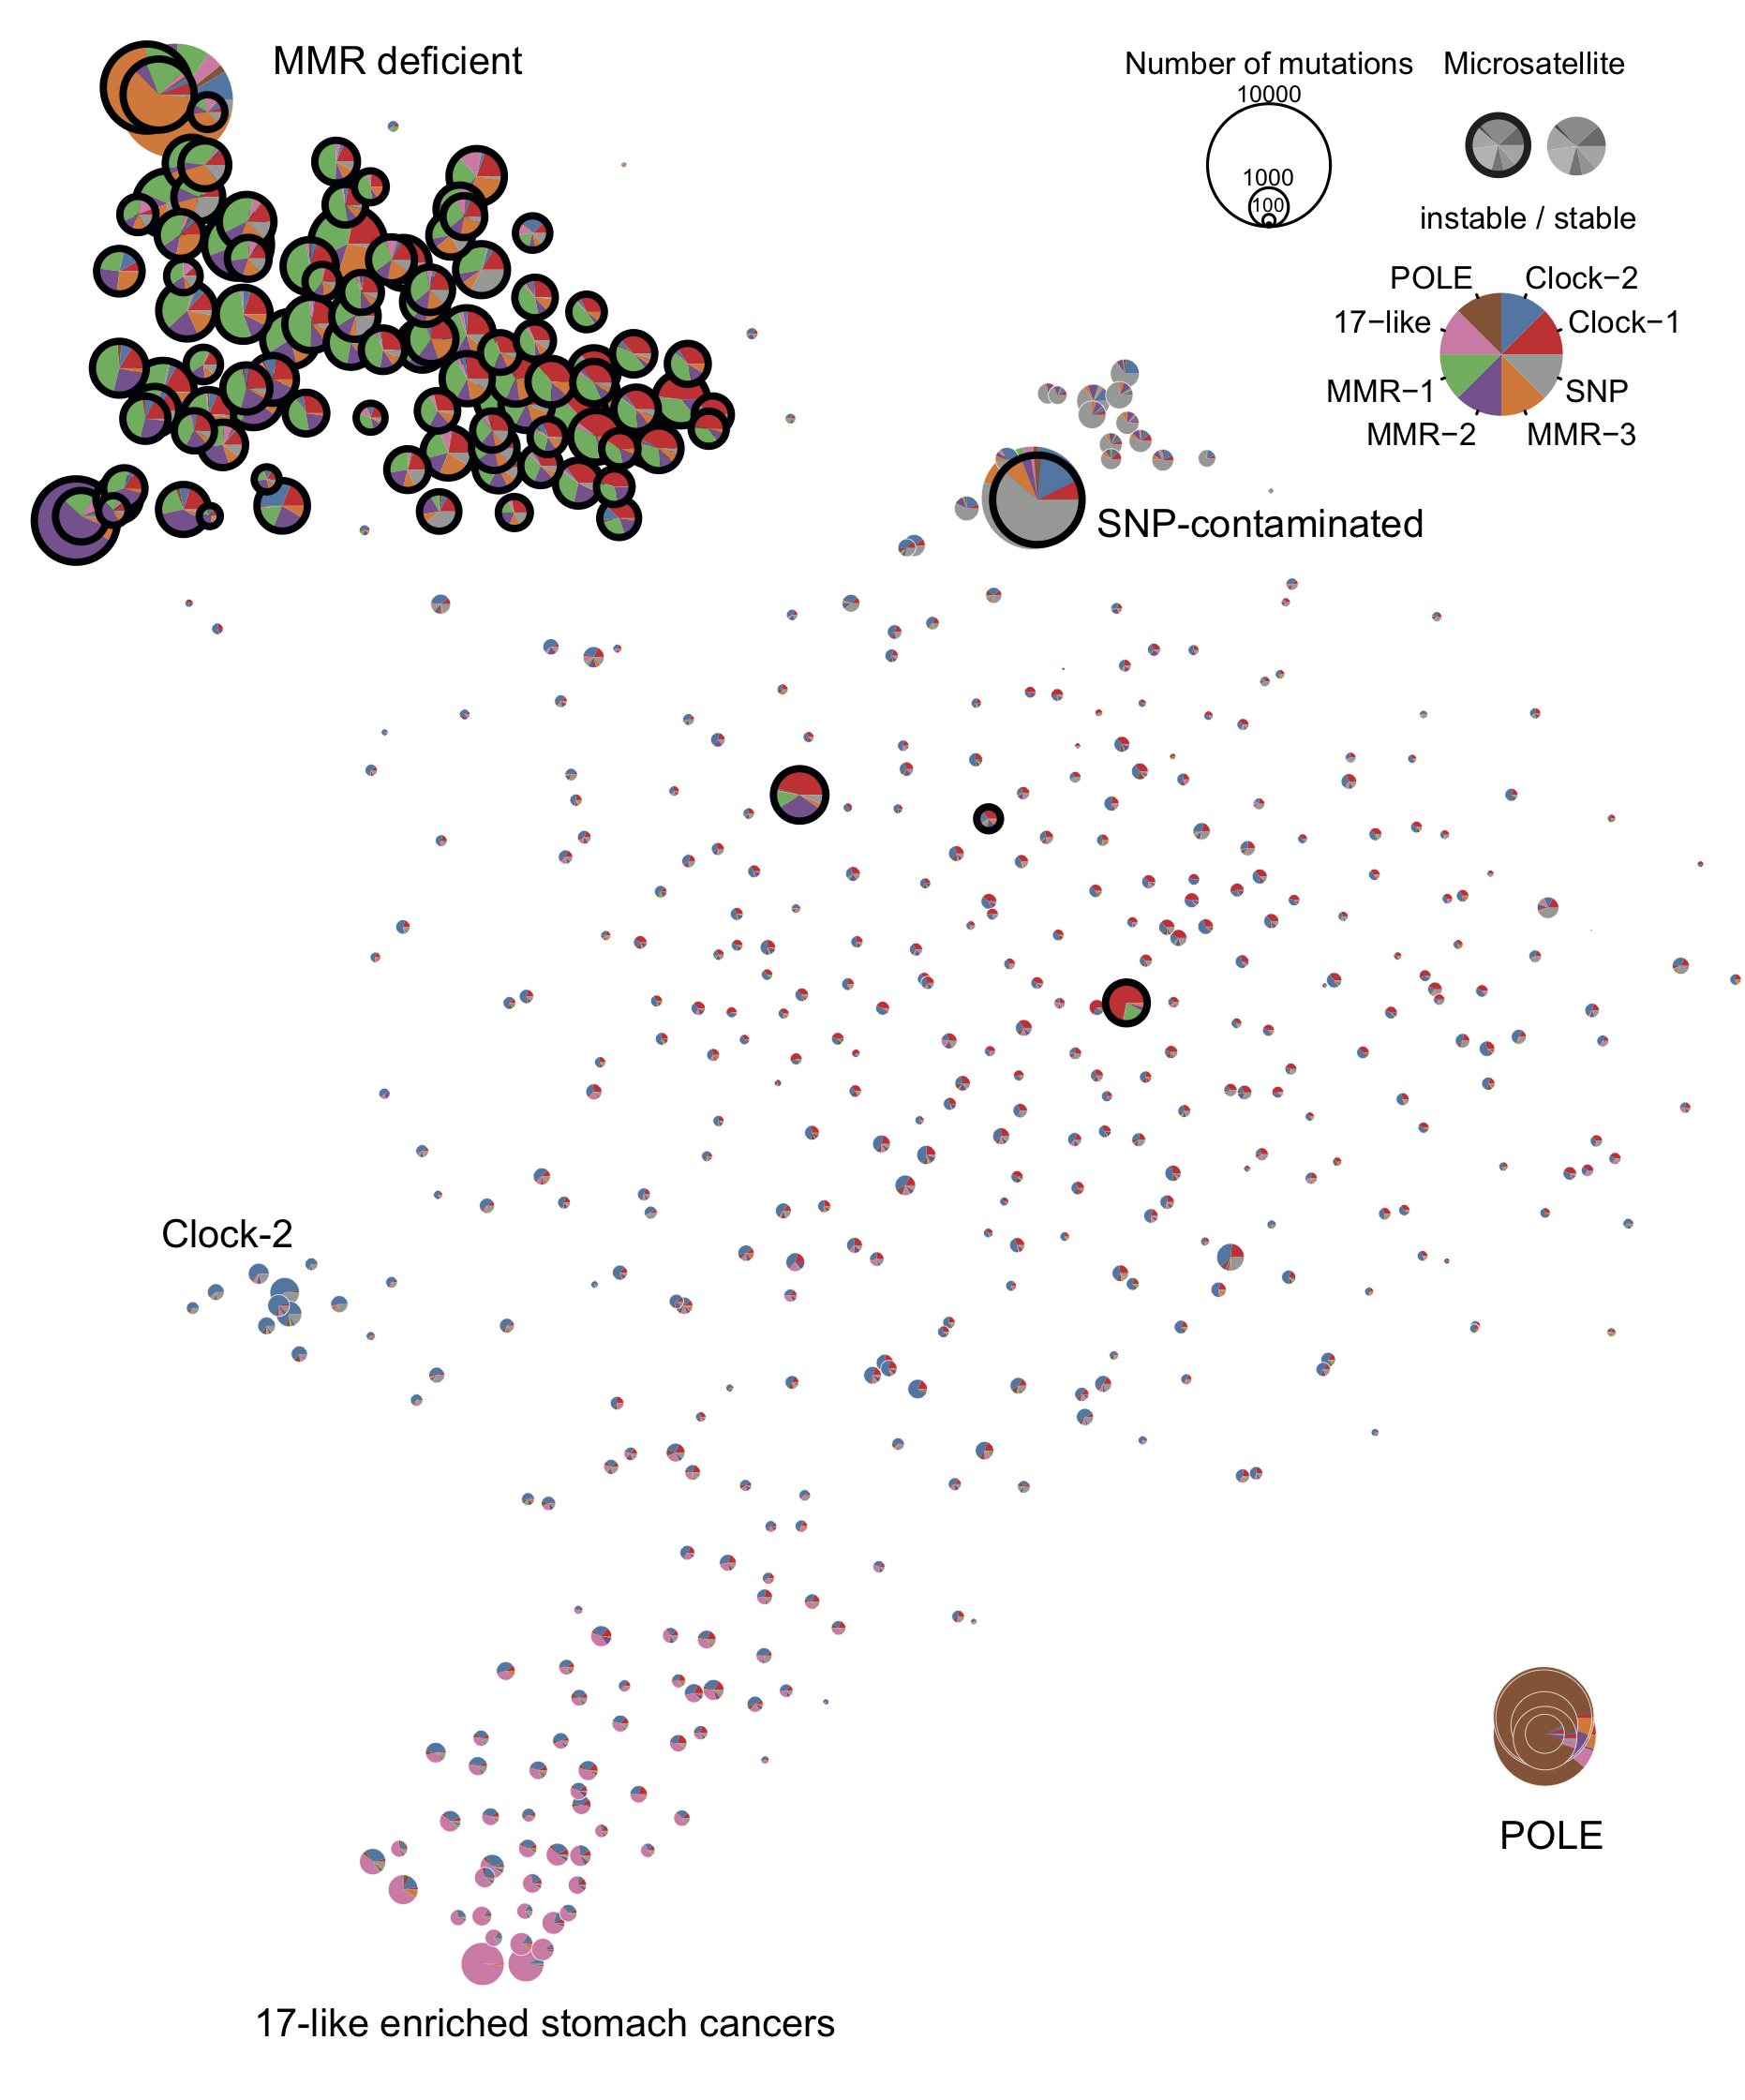
\includegraphics[width=1\textwidth]{figures/COAD_STAD_tsne.png}}
  \caption{Similarity map of mutational spectra in stomach and colorectal cancers. Each circle represents a sample, its radius reflects the number of mutations, and the color segments correspond to the signature decomposition.}
  \label{COADtsne}
\end{figure}

By plotting a map of similarities between mutational spectra of all samples using a t-SNE 
representation \cite{Maaten2008-de}, we have observed some distinctive grouping of samples
(Figure \ref{COADtsne}). A small yet very secluded cluster was formed by the samples
whose mutational spectra were defined by POLE signature (brown). Samples dominated
by Clock-2, 17-like or SNP signature tended to point out at different ends of the
map (blue, pink and grey, respectively).

The majority of MSI samples (circles with a black rim) concentrated in one cluster. These samples carried
diverse combinations of signatures MMR-1-3 and Clock-1, but overall this group was mostly defined by
the presence of the MMR-1 signature (green), while the MMR-2 (purple) and MMR-3 (orange) signatures occurred
in a small number of tumours with high mutation burden. Moreover, the samples with highest number of 
mutations were in fact largely described by a single signature, possibly reflecting the tendency of 
signature reconstruction method to extract signatures from the most extreme cases first, and
then fit them to other samples.


%%%%%%%%%%%%%%%%%%%%%%%%%%%%%%%%%%%%%%%%%%%%%%%%%%%%%%%%%%%%%%%%%%%%%%%%%%%%%%

\subsection{Mismatch repair and its interactions with other processes}

Individual signatures often represent the most extreme ends of the mutational spectrum; 
a typical tumor, however, is usually represented by a linear combination of multiple processes. 
Given the different substrate specificities of MutS-$\alpha$ and MutS-$\beta$, 
MMR-2 and MMR-3 might reflect mutations arising by an inactivation of unique subunits within 
these heterodimers. However, investigating MMR gene mutations and methylation status 
in these tumor samples, we observed few cases of MSH6, MSH3, PMS1 and MLH2 inactivation, which 
often occurred in combination with inactivation of other MMR genes, but the numbers were
too low to infer any conclusion.

In addition to the MMR-1-3 signatures, MSI samples were also partially composed by signature
Clock-1. The Clock-1 signature closely resembled COSMIC signature 1, which was associated with 
5-methyl-cytosine deamination and found to be correlated with the age at the time of diagnosis 
across a range of cancer types (\cite{Alexandrov2013-md},\cite{Alexandrov2015-clock}). Given that there was no difference in the 
average age between MMR deficient and proficient groups of samples, this signature should be
contributing a similar amount of mutations across these two groups. Since the average mutational 
burden in MMR deficient samples is higher, relative contribution of Clock-1 to these samples 
should be lower. However, we observed no change in the relative contribution, and a 10-fold
increase (one-tailed t-test p-value $= 4.3 \cdot 10^{-22}$) in the absolute number of 
mutations assigned to Clock-1 in MMR deficient samples compared to proficient, 
similarly to signatures directly associated with MMR status (Figure \ref{clock1}).

\begin{figure}[h]
  \centering
  \centerline{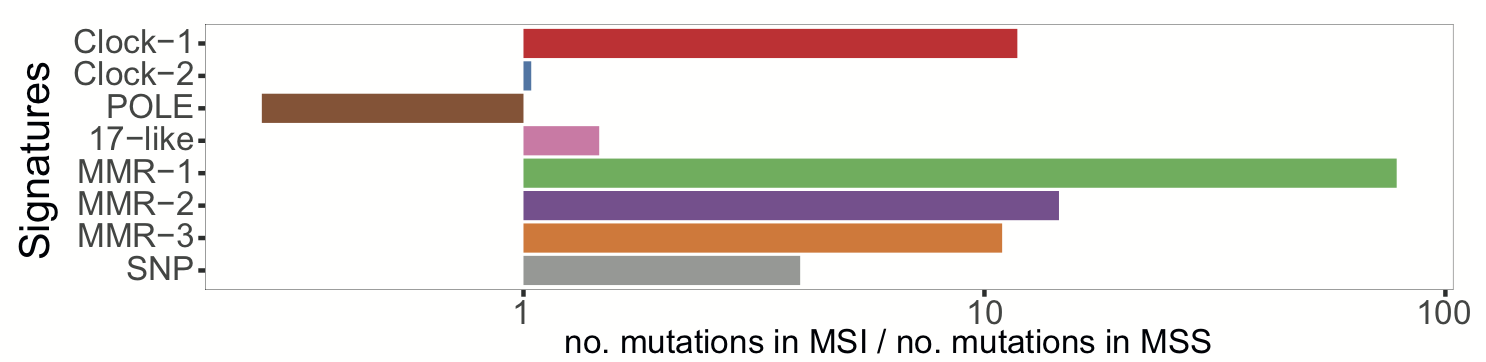
\includegraphics[width=1\textwidth]{figures/clock1_in_MSI.png}}
  \caption{Fold change in number of mutations contributed by different signatures in MSI and MSS samples.}
  \label{clock1}
\end{figure}

This relationship indicates that MMR deficiency increased the rate of mutations resulting from 
spontaneous cytosine deamination.
\todo[inline]{Explain in more detail the non-canonical mismatch repair - replication independent!}
A number of studies have previously suggested an interaction between base excision repair 
and mismatch repair pathways in the repair of G:T mismatches caused by cytosine deamination (\cite{Bellacosa2001-uf}, \cite{Tricarico2015-px}, \cite{Grin2016-cw}),
so-called non-canonical mismatch repair. Notably, two of the COSMIC signatures associated with MMR deficiency, 
signatures 6 and 20, are very similar (cosine similarity 0.97) and only differ in the contribution 
of C$>$T mutations in NCG context, which may be reflecting a mixture between MMR mutational footprint
and acceleration of cytosine deamination.

%%%%%%%%%%%%%%%%%%%%%%%%%%%%%%%%%%%%%%%%%%%%%%%%%%%%%%

\subsection{Deletions and insertions in repetitive sequences}

Distribution of 1-bp indels extracted alongside with the base substitution profile for signature MMR-1 favours 
all of the bases equally (Figure \ref{COADsigs}), however in \textit{C. elegans} we observed a huge shift 
towards indels of A and T. Mainly, this is due to a difference in homopolymer composition between the two 
systems: homopolymer pool in \textit{C. elegans} genome consists mostly of poly-A and poly-T stretches
(Figure \ref{worm_homo}), whereas the human exome features equal amounts of homopolymers formed by 
different bases (Figure \ref{human_homo}). In total, human exome contained 976,390 homopolymer stretches 
between 4 and 43 bases in length, with A/T homopolymers contributing only about 55\% or all homopolymers. 
For comparison, \textit{C. elegans} genome (with length of 100 Mbps, approximately 3 times larger than human exome) 
contained 3,433,785 homopolymers of which 94\% were A/T stretches.

\begin{figure}[h]
  \centering
  \centerline{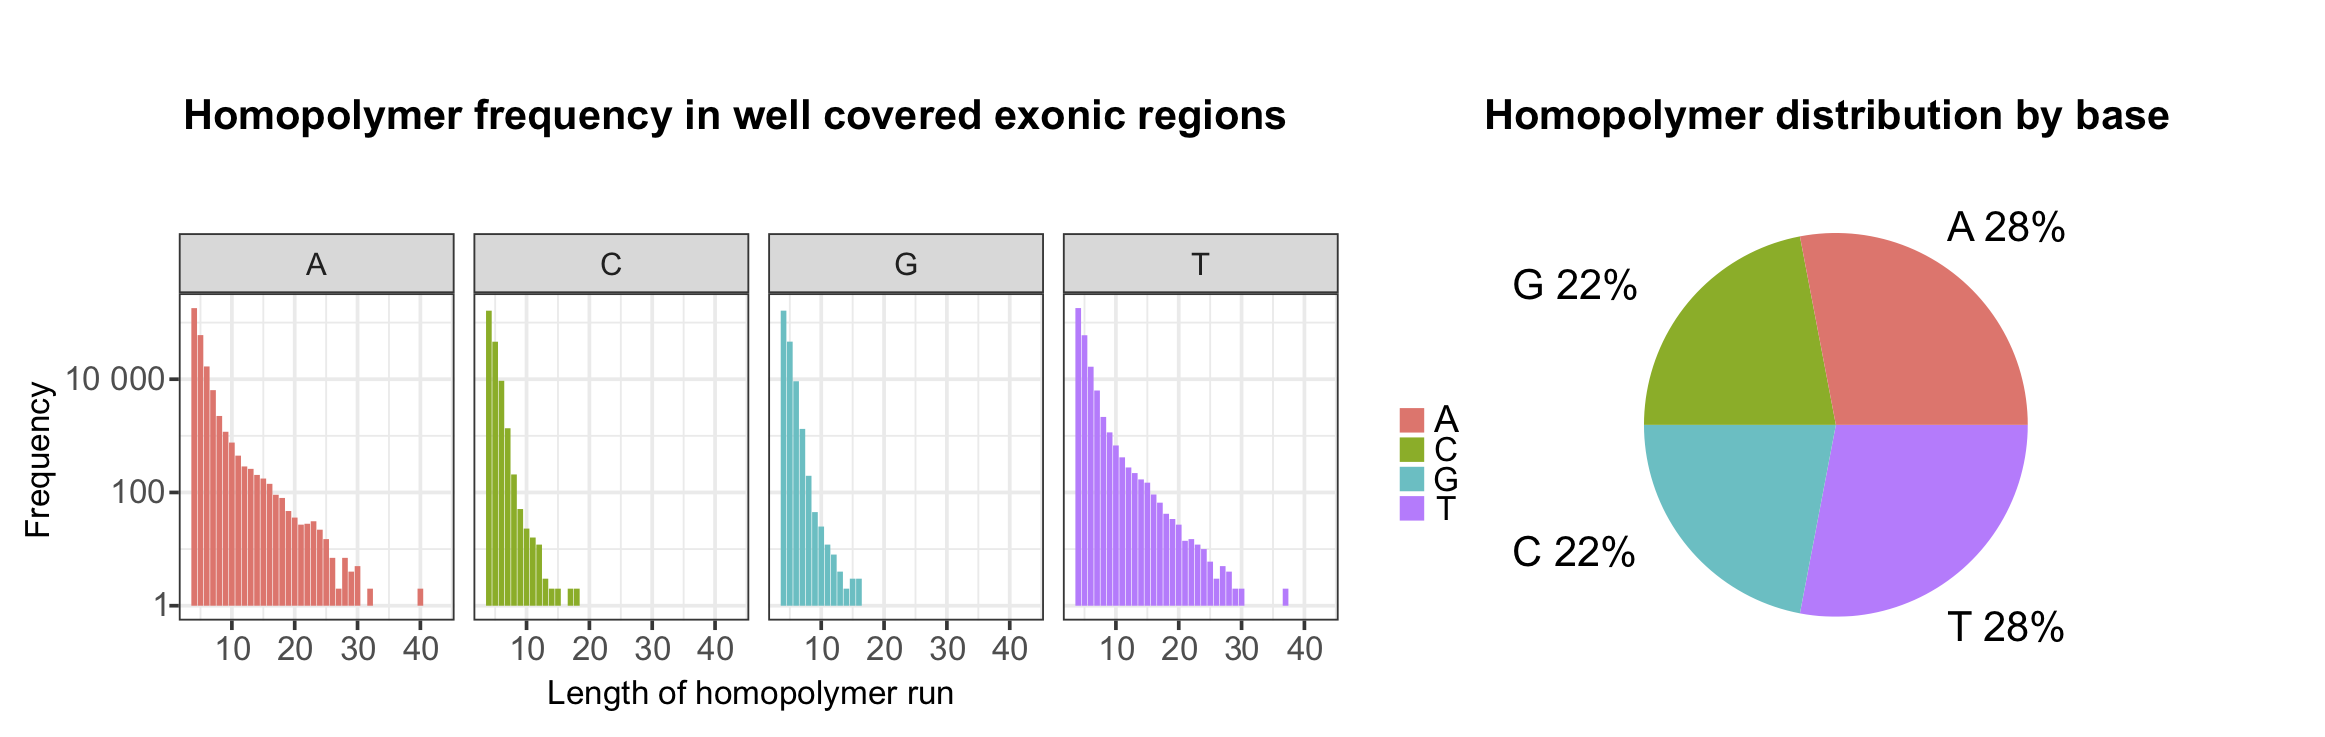
\includegraphics[width=1\textwidth]{figures/human_exome.png}}
  \caption{Distribution of homopolymeric sequences in human exome.}
  \label{human_homo}
\end{figure}

When adjusted for the difference in the available span of homopolymers, the frequencies of 
indels of A and T in \textit{C. elegans} \textit{mlh-1} and \textit{pms-2} knockouts were still about 4 times higher that those of G and C (Figure \ref{worm_vs_human}). This indicates intrinsic differences in the processing of deletions and insertions of single bases which may be related to such 
features as transcriptional activity or the distance to origins of replication.

Overall, 82\% (25,093 out of 30,561) indels in the human dataset were single base indels, and the majority of these occured in homopolymer runs: 69-72\% of 1 bp indels/sample in the COAD dataset and 91-93\% 1 bp indels/sample for STAD (Figure \ref{stad_coad_homo}). 

\begin{figure}[h]
\subfloat[A]{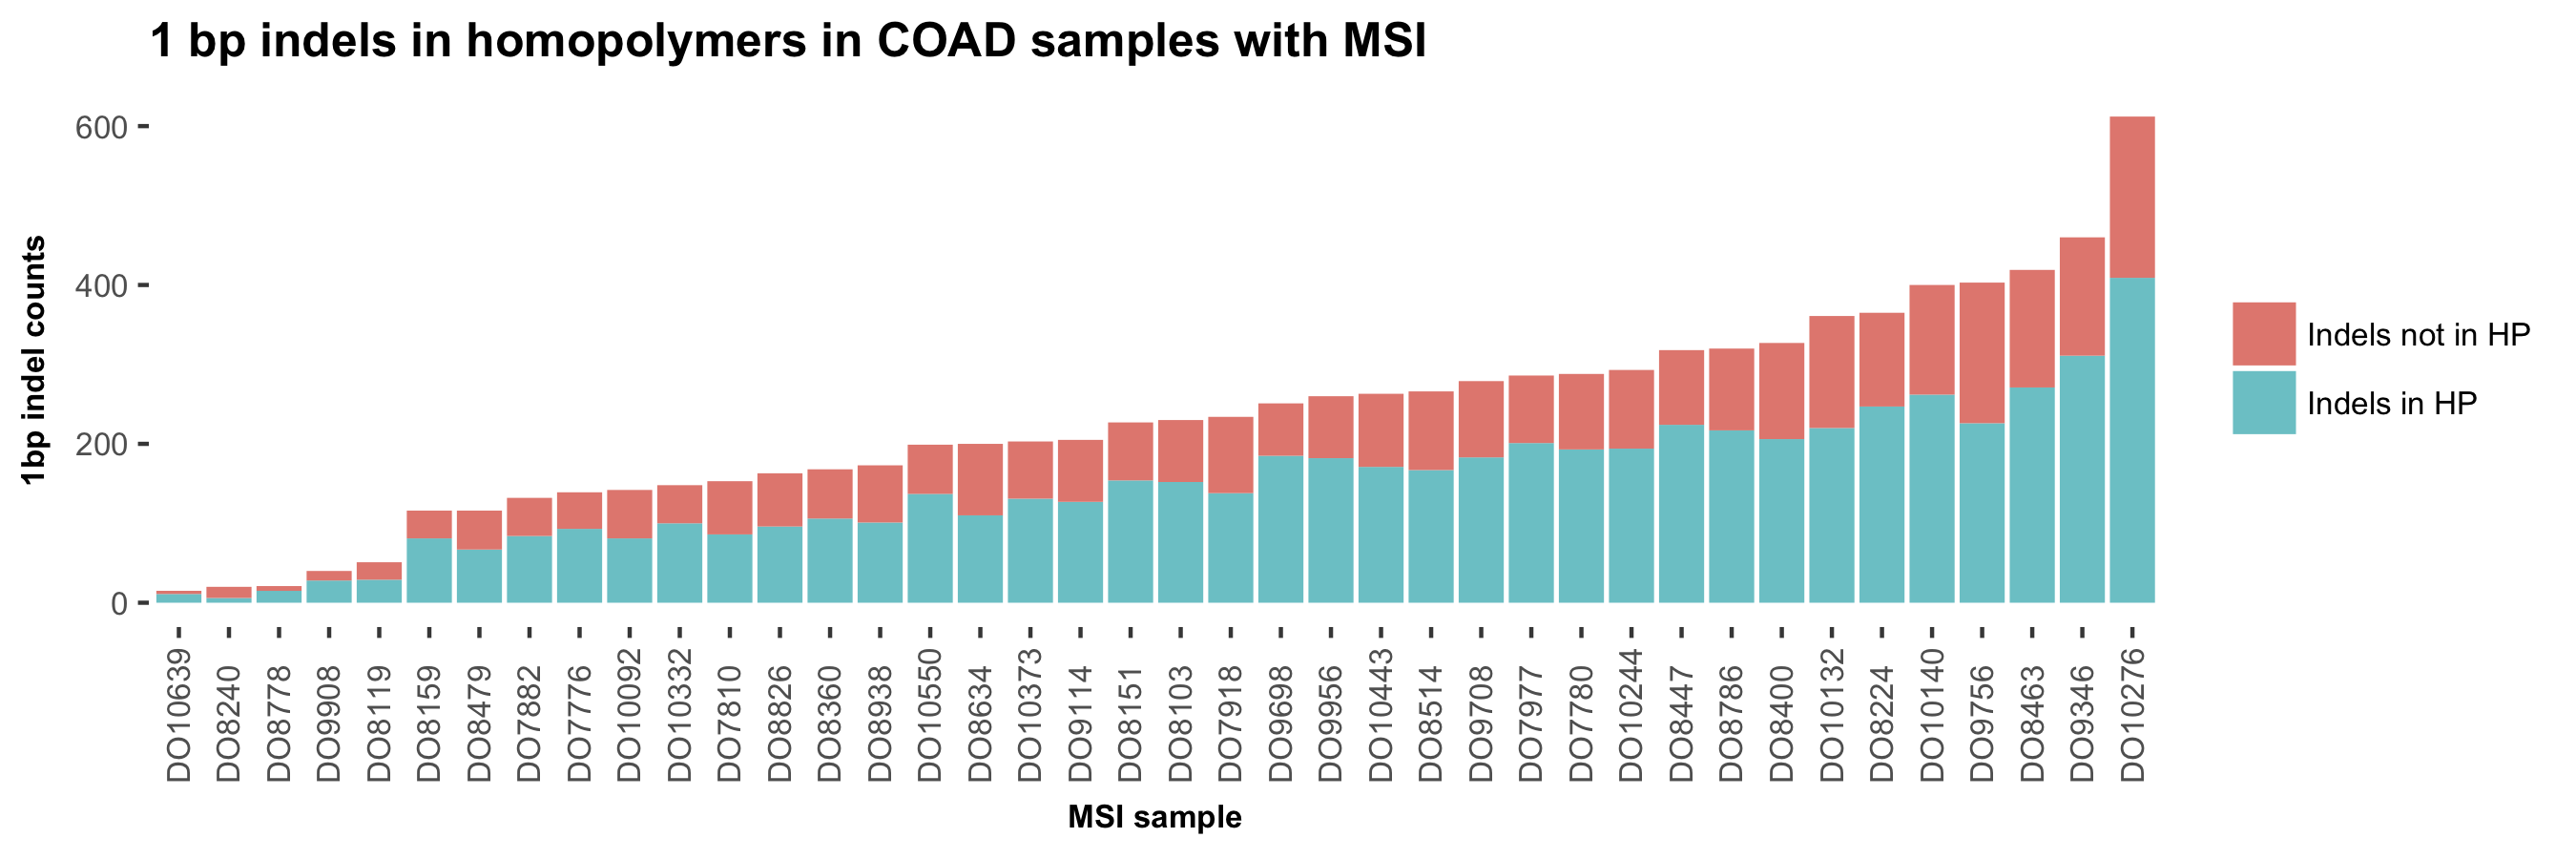
\includegraphics[width = 1\textwidth]{figures/coadindelsinhomopolymers.png}}\\
\subfloat[B]{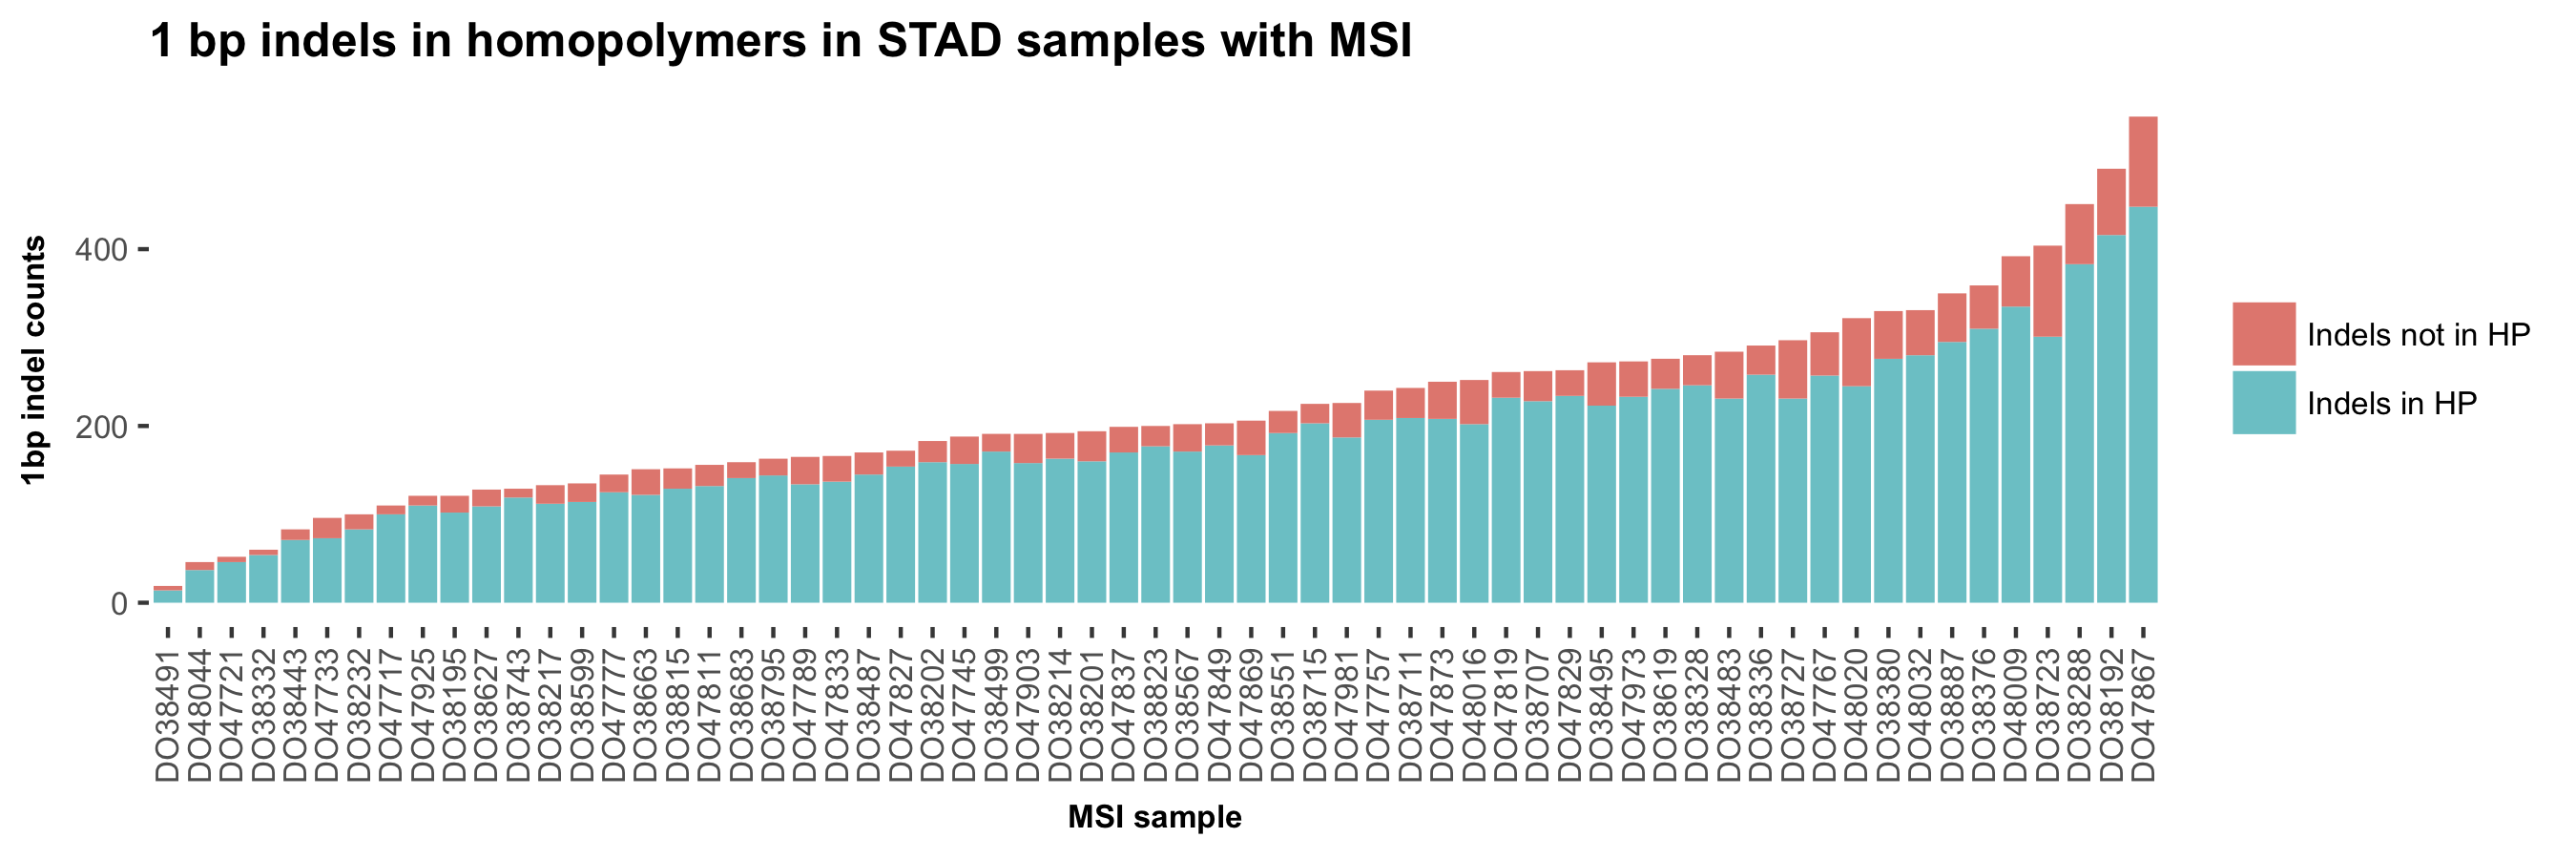
\includegraphics[width = 1\textwidth]{figures/stadindelsinhomopolymers.png}}
\caption{Indels in (blue) and outside (red) of homopolymeric regions per sample in A) COAD and B) STAD dataset.}
\label{stad_coad_homo}
\end{figure}

Total amount of indels per homopolymers relative to the number of homopolymers in 
human data was much lower than that in \textit{C. elegans},
hence analysing the frequencies of indels per homopolymers of different length deemed infeasible.

%%%%%%%%%%%%%%%%%%%%%%%%%%%%%%%%%%%%%%%%%%%%%%%%%%%%%%

\section{\textit{C. elegans} experimental MMR deficiency signatures correspond to MMR-1 signature in cancers}

Having the mutational spectra of \textit{mlh-1} and \textit{pms-2} mutants and
\textit{pole-4; pms-2} double knockout acquired in \texit{C. elegans} experiments
at hand, we aimed to check how comparable are these signatures to the one active 
in cancer genomes. Using the trinucleotide frequency correction introduced in Chapter 2,
we brought the \textit{C. elegans} signatures in accordance with human exome (using the counts from \cite{Rosenthal2016-hq}).

\begin{figure}[h]
  \centering
  \centerline{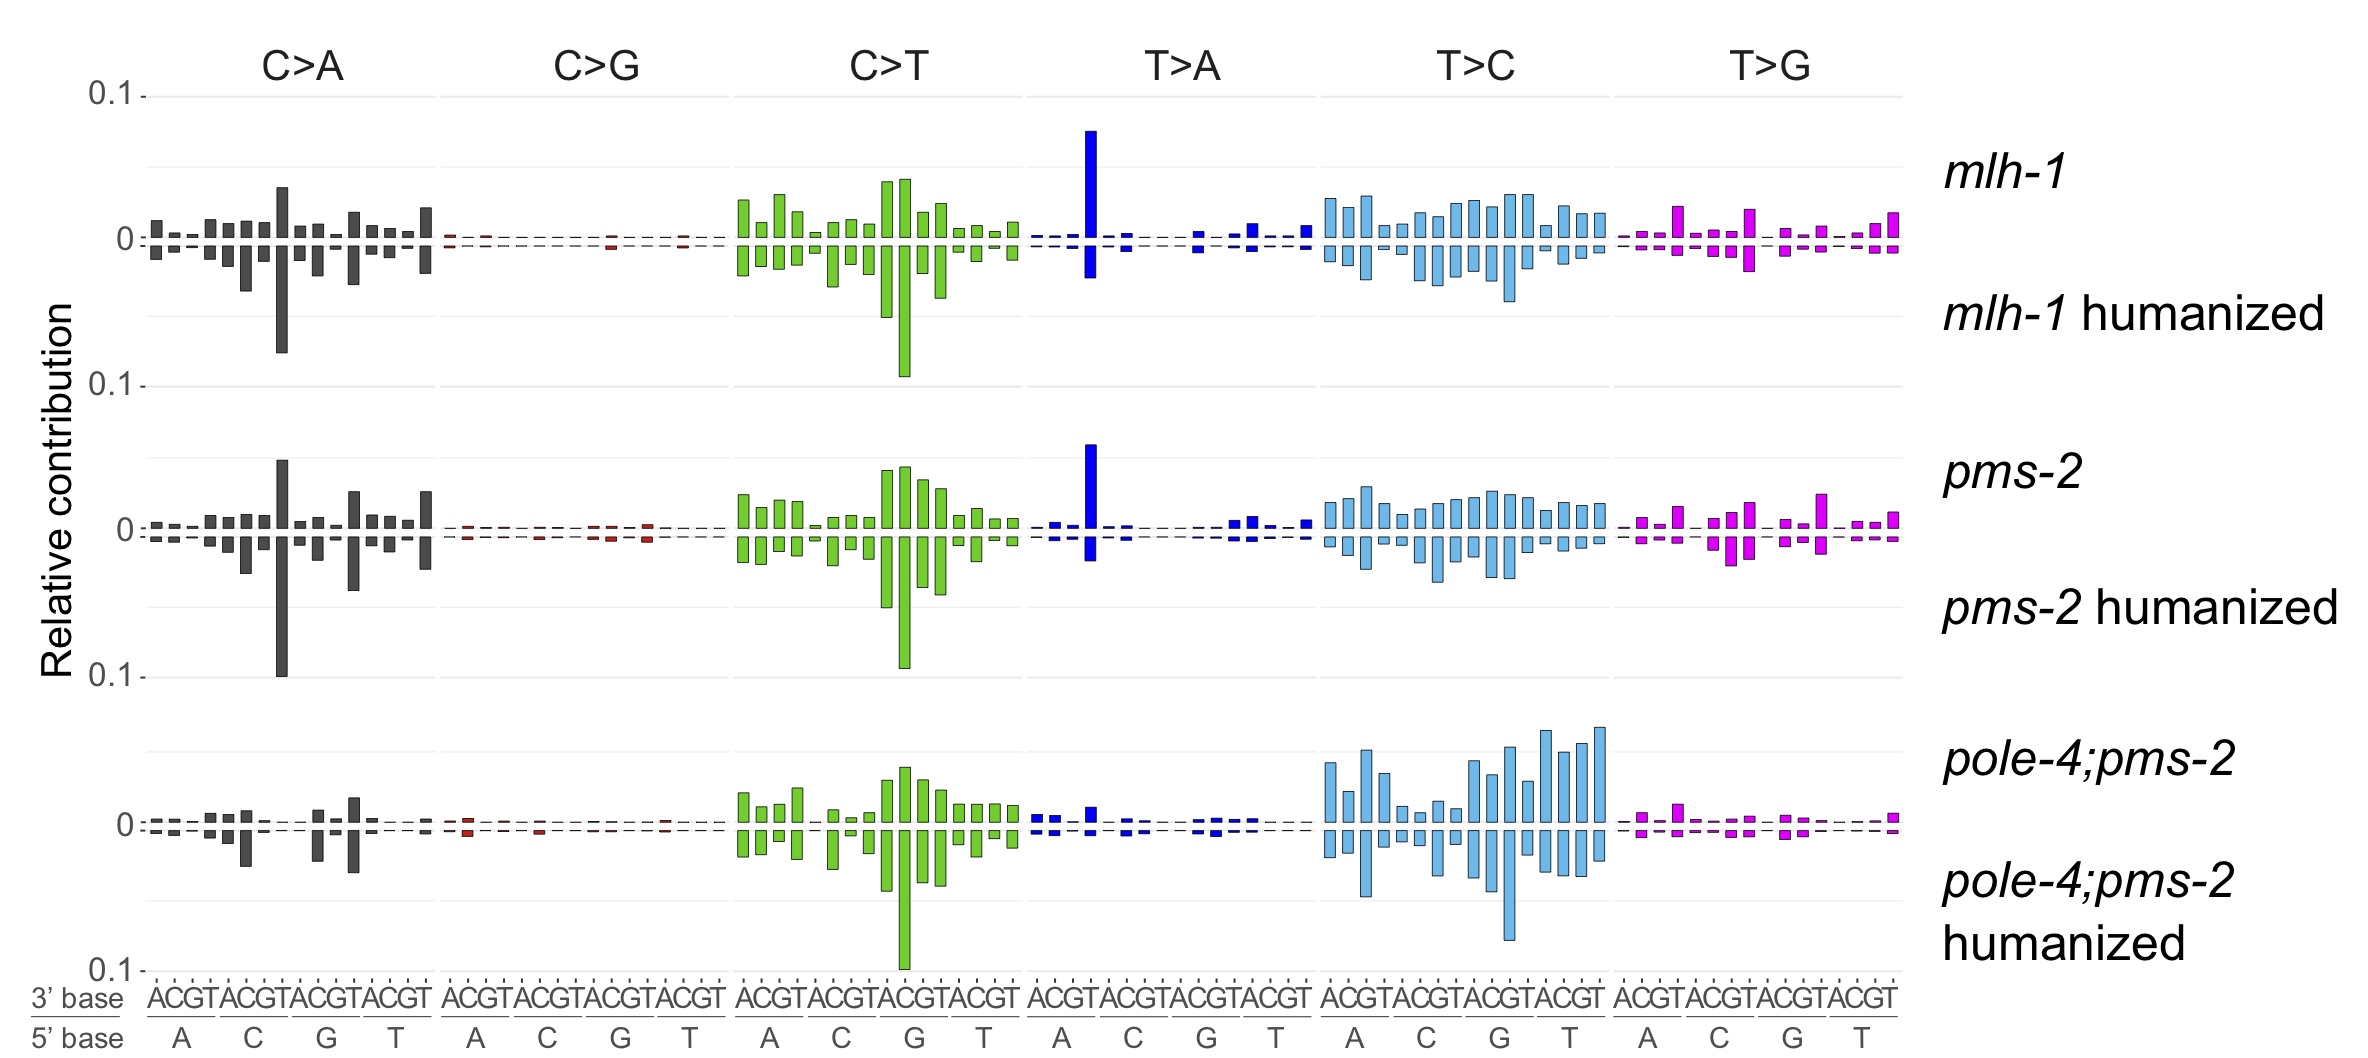
\includegraphics[width=1\textwidth]{figures/mmr_mutational_patterns_for_c_elegans_humanisation.png}}
  \caption{Original and humanized versions of \textit{C. elegans} experimental signatures of \textit{mlh-1}, \textit{pms-2} and \textit{pole-4; pms-2} knockouts.}
  \label{humanized_mmr}
\end{figure}

Of the three human MMR-associated de novo signatures, only MMR-1 displayed 
similarity to \textit{C. elegans} MMR substitution patterns with cosine 
similarities of 0.84 and 0.81 to \textit{pms-2} and \textit{mlh-1} signatures, 
respectively (Table REF, Figure \ref{worm_vs_human}). Most of the discrepancy 
between the \textit{C. elegans} MMR deficiency spectra and MMR-1 was coming 
from different levels of CpG$>$TpG mutations and change in frequency of ATT$>$AAT mutations.

\begin{figure}[h]
  \centering
  \centerline{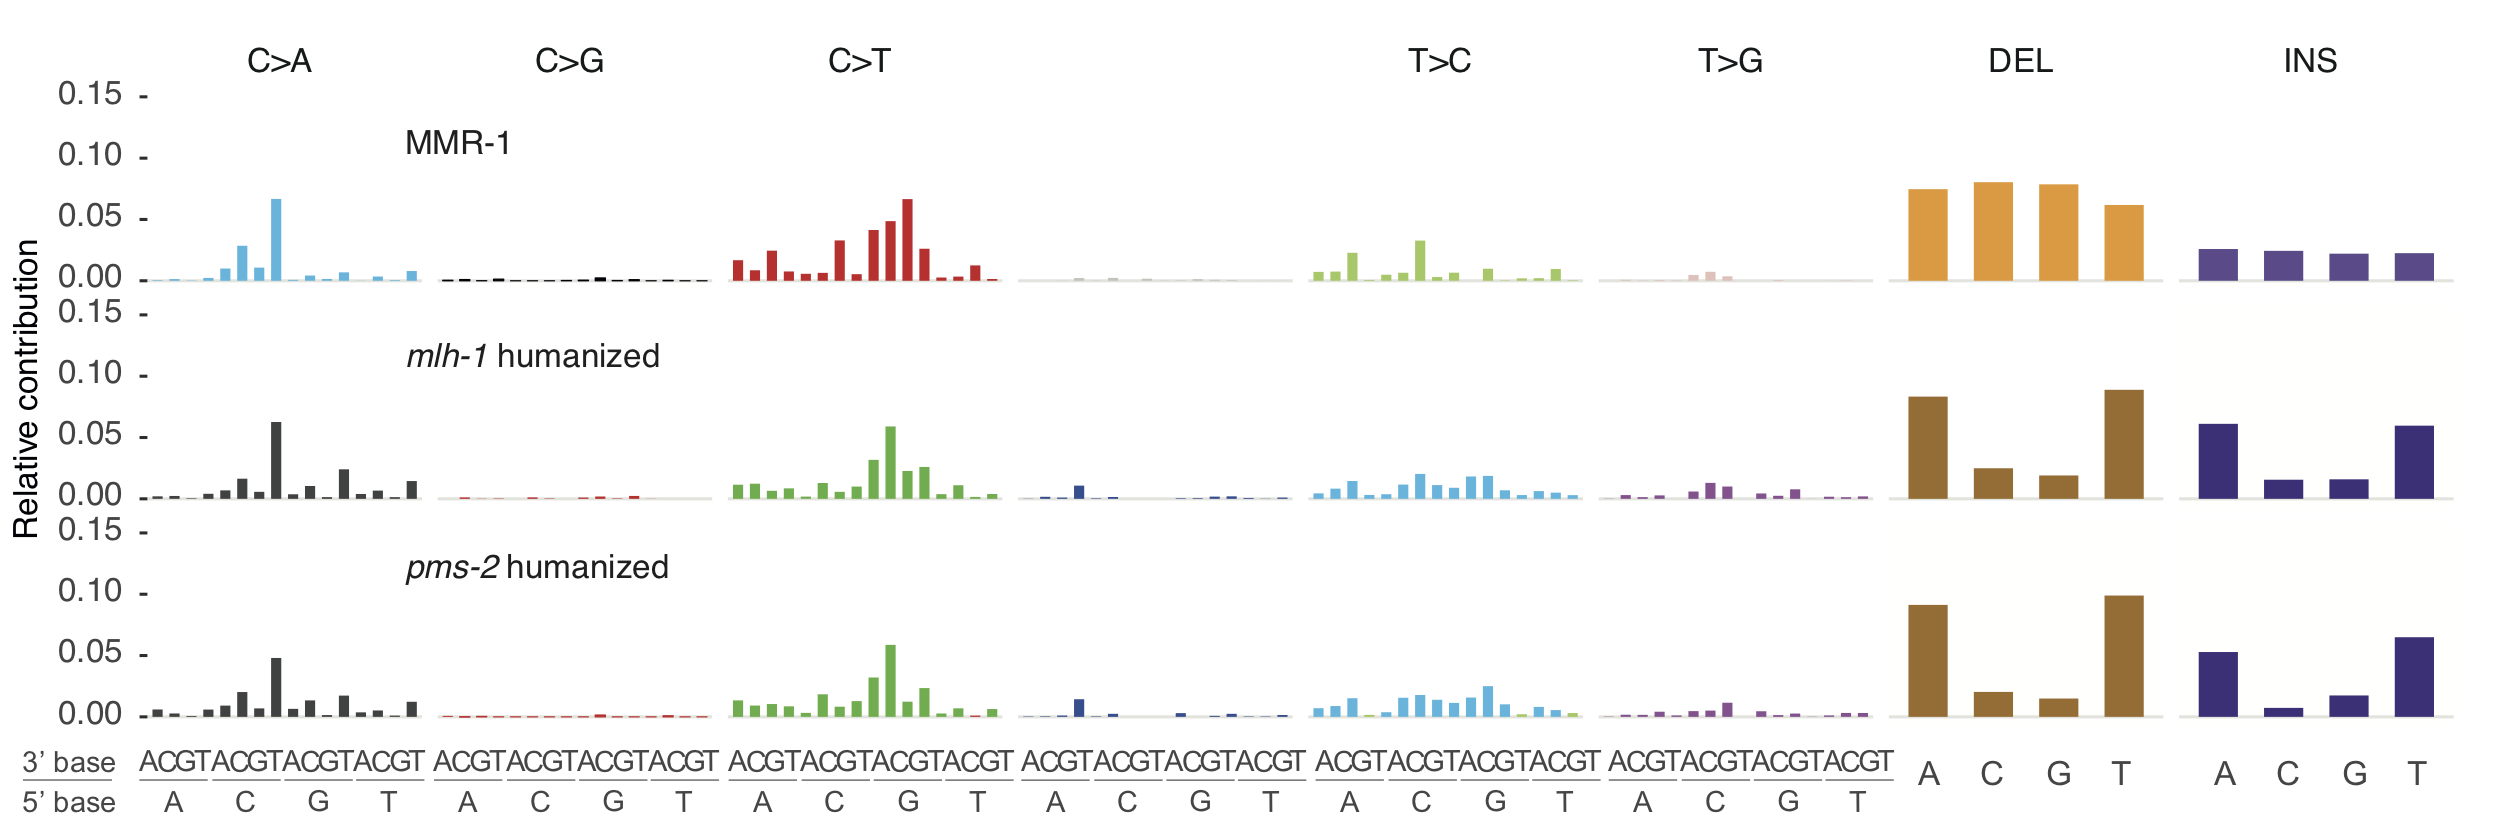
\includegraphics[width=1\textwidth]{figures/worm-human-mmr-sig.png}}
  \caption{Trinucleotide context comparison between \textit{C. elegans} genome and \textit{H. sapiens} exome.}
  \label{worm_vs_human}
\end{figure}

\textit{C. elegans} is lacking 5-methyl-cytosine (\cite{Greer2015-im}), hence there is no
spontaneous deamination, which explains mcuh lower levels of C$>$T mutations at CpG sites.
If these contexts were excluded, MMR-1 would show similarities of 0.92 to \textit{pms-2} 
knockout signature, and 0.90 to \textit{mlh-1} knockout signature. Human exome and 
\textit{C. elegans} genome also have different composition of homopolymers in 
different bases. Amount of poly-A and poly-T in \textit{C. elegans} genome is 
much higher despite a comparable size (30 Mbps of human exome, and 100 Mbps of 
worm genome), hence the probability of clashes between A-homopolymers and 
T-homopolymers is higher. Detection of indels at such positions is difficult 
since a variant caller would easily mistake a deletion of a T or insertion of 
an A for a T$>$A transversion.

\begin{wrapfigure}{r}{0.5\textwidth}
  \centering
\centerline{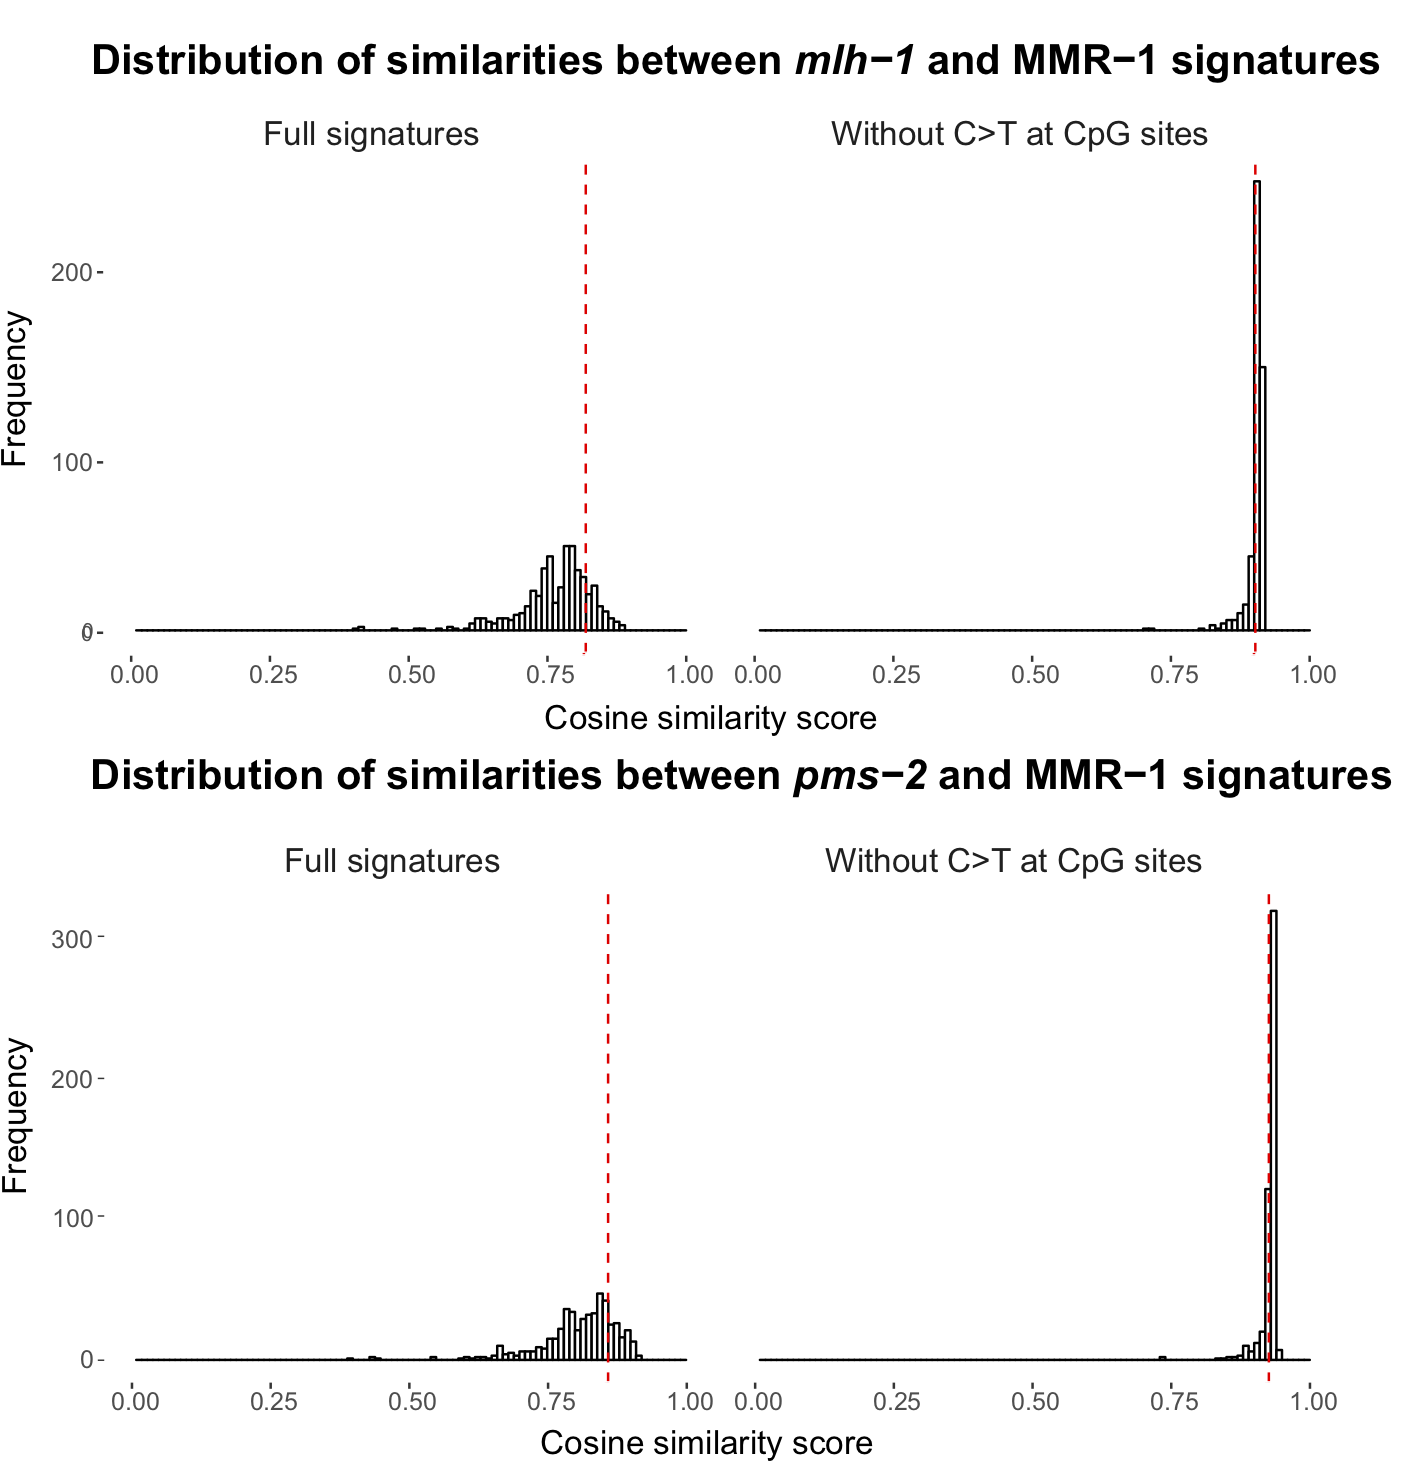
\includegraphics[width=0.5\textwidth]{figures/simulating_signature_variability_worm_human.png}}
  \caption{Distribution of similarities between humanized \textit{mlh-1} signature (top) or \textit{pms-2} signature (bottom) and human de novo signature MMR-1 with and without NCG$>$NTG mutations.}
  \label{similarity_sim_worm_human}
\end{wrapfigure}

Due to statistical challenges of separating correlated processes (such as MMR deficiency and 5meC deamination),
we measured the uncertainty of signature comparison. Stability assessment of the similarity score between 
\textit{C. elegans} signatures and MMR-1 was performed by calculating similarities of random draws 
from \textit{C. elegans} signatures' 95\% confidence intervals and signature most similar to MMR-1 
among the ones calculated for each jack-knife (leave-one-out) bootstrapped sample of 
the COAD/STAD dataset (Figure \ref{similarity_sim_worm_human}).

Stability assessment of the similarity score between \textit{C. elegans} and human signatures shows that 
the similarity between humanized MMR patterns and MMR-1 signatures varies substantially 
(inter-quantile range (IQR) of 0.66 to 0.76 for \textit{mlh-1} and 0.70 to 0.80 for \textit{pms-2}, respectively), 
but shrinks as soon as we exclude C$>$T at CpG sites (IQR of 0.87-0.90 and 0.90-0.92, respectively) 
(Figure \ref{similarity_sim_worm_human}).
None of the human signatures showed notable 
similarity to the \textit{pole 4; pms-2} mutation pattern.

%%%%%%%%%%%%%%%%%%%%%%%%%%%%%%%%%%%%%%%%%%%%%%%%%%%%%%%%%%%%%%%%%%%%%%%%%%%%%%

\section{Discussion}

In this chapter, we characterized the mutational signatures of mismatch repair deficiency across colorectal and stomach cancers, and compared those to the mutational landscapes associated with MutL MMR in \textit{C. elegans}. MMR deficiency was of a special interest as it leads to the highest number of mutations and the most distinctive phenotype compared to other DNA repair deficiencies in our screen, surpassed only by that of the \textit{pole-4}; \textit{pms-2} double mutants which exhibited 2-3 fold higher mutation rates. In addition to high substitution burden, MMR deficiency was associated with a high number of small indels in repetitive regions in both \texit{C. elegans} and human cancers, consistent with the concept of polymerase slippage on homopolymer stretches which should normally be repaired by the MMR system. 

Out of the signatures we found to be associated with microsatellite instability in cancer cells, only one signature (MMR-1) was shown to be related to the experimental signatures of MMR deficiency found in \textit{C. elegans} \textit{mlh-1} and \textit{pms-2} mutants. Taking into account the controlled nature of the \textit{C. elegans} experiment, we postulated that MMR-1 may in fact reflect the underlying "basal" mutational process of DNA replication errors repaired by MMR conserved between species. Consistent with this, we find that MMR-1 showed high correlation with  MSI status, and performed well in tumour classification (P-value $4.7 \cdot 10^{-55}$ , AUC 0.985) into mismatch repair deficient and proficient. Similarly, another study using human $MLH1^{KO}$ organoid cells identified a mutational profile similar to that of MMR-1 \cite{Drost2017-dl}.

The distribution of signature contribution indicates mixed origins of the other two MSI-associated signatures which tend to be concentrated in the most hypermutated samples. These signatures might be caused by a defect in another DNA repair gene, which leaded to amplification of damage created by replicative polymerases, or a defect in replicative polymerase itself which contributed to the change of error profile, similar to \textit{pole-4}; \textit{pms-2} double mutants in \textit{C. elegans} experiments or COSMIC signature 14 which was found to be associated with concurrent loss of MMR and POLE proofreading ability \cite{Haradhvala2018-ma}. Similarly, even the most common signature of human MMR deficiency (MMR-1) also included an element of failing to repair C$>$T changes linked to CpG demethylation -- a process that does not occur in \textit{C. elegans}, which was contributing at a higher degree to MSI samples due to the secondary role of MMR machinery in the repair of deaminated 5-me-C.

In the next chapter, I will move on to the part of the screen which combined DNA repair deficiency with mutagen exposure, and present the concept of genotype-mutagen interaction. I will present ht model for quantifying non-additive effect with arbitrary direction (both positive and negative), show the abundance of significant damage-repair interaction effects throughout the screen, and investigate its relevance to the analysis of cancer genomes.

\end{document}

%\textit{Comparison of signature contributions}

%Relative and absolute contributions of every signature to the samples from the united dataset were tested for association with MSI/MSS status using one-tailed Student t-test. All p-values were adjusted for multiple testing correction using Bonferroni procedure.

%COSMIC signatures were also adjusted to exome nucleotide counts as they were mostly derived from whole exomes (Alexandrov et al. 2013a; Alexandrov et al. 2013b) and the comparison of de novo signatures to COSMIC is more valid in exome space (Suppl. Doc1?). All signatures were further normalized so that the vector of probabilities sums up to 1 (Supplemental Data 1). 

%Analysis of mutations in 
%MMR-related genes MLH1, PMS2, MSH2, MSH3, MSH6, PMS1, MLH3 and EPCAM (\cite{Hsieh}, %\cite{Ligtenberg}) consisted of identification of high-impact mutations (missense, 
%frameshift or splice region variants, disruptive in-frame deletions or insertions, stop gained,% 
%start lost, and stop lost) in the genes of interest. Hypermethylation of MLH1 was defined by 
%correlating the methylation values of 43 CpG sites in the CpG island overlapping the MLH1 gene 
%promoter with MLH1 expression level. Expression and methylation data for the two cohorts are 
%also available in ICGC database.